\appendix
\section{Appendix}
\subsection{Short summary of the LAR scheme}


\begin{figure*}[!htbp] % figure placement: here, top, bottom, or page
 \centering
 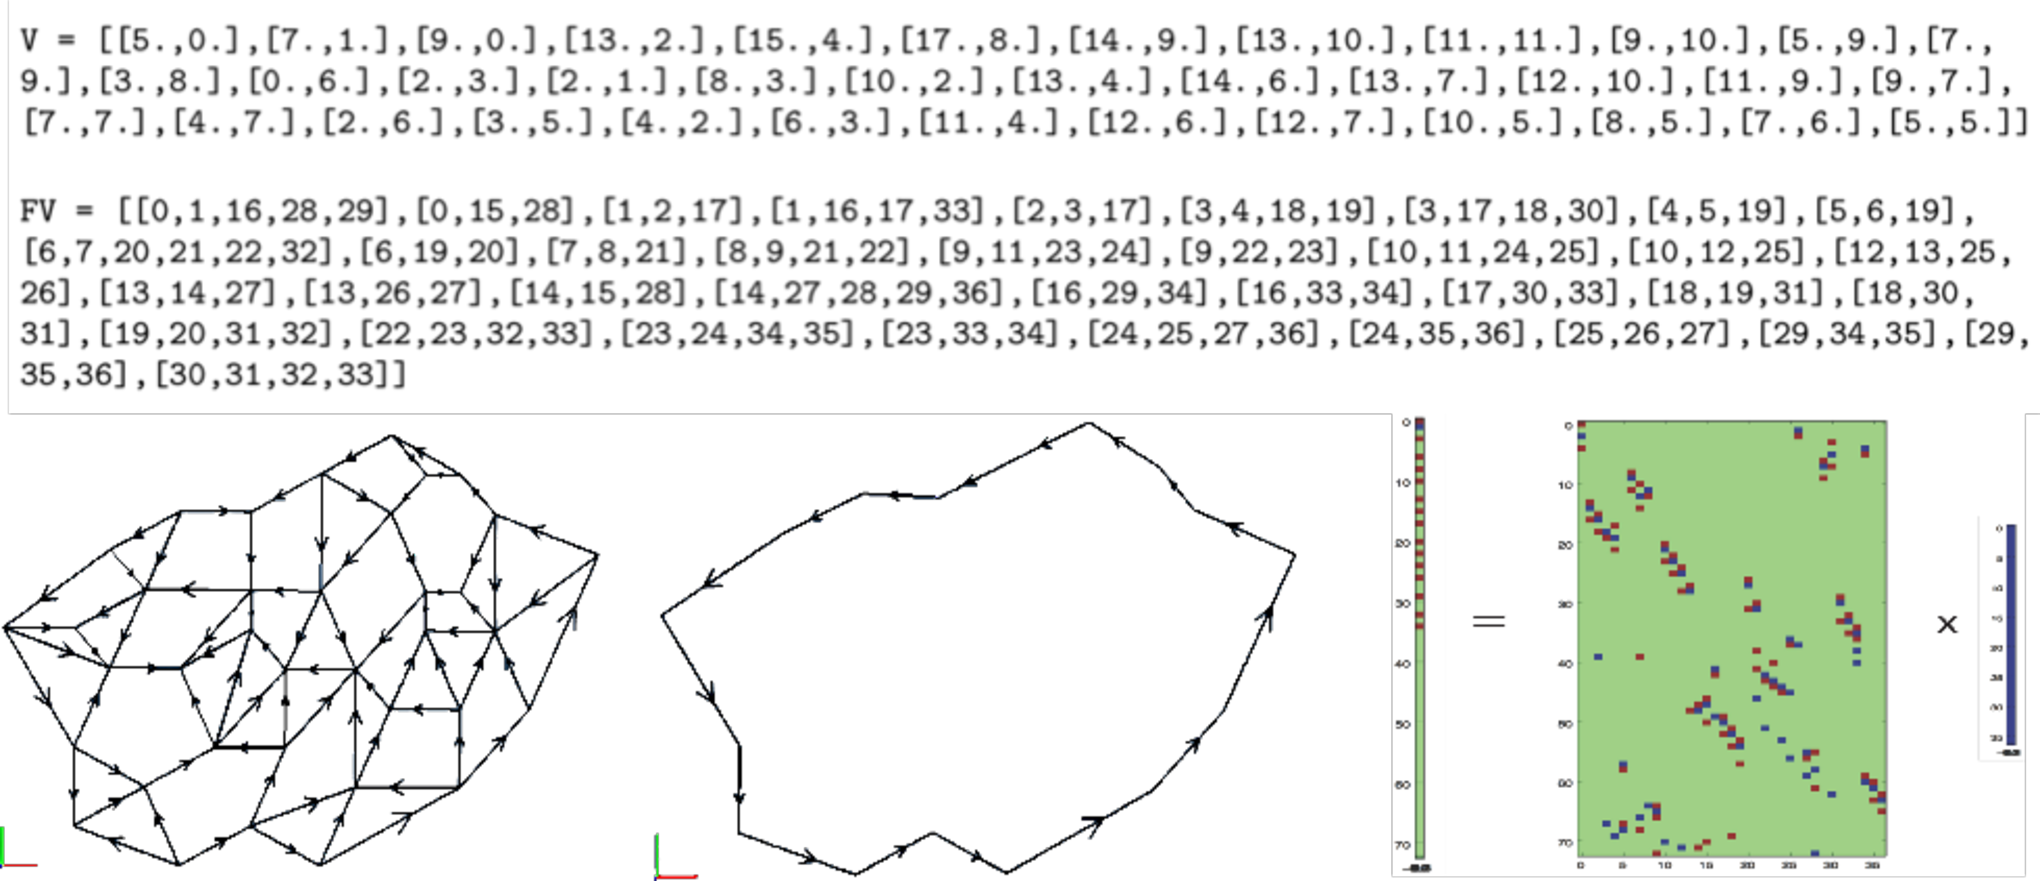
\includegraphics[width=\linewidth]{images/minimum} 
 \caption{A toy example of the LAR scheme: (a) the bare minimum of data with \emph{complete} information about topology; (b) the extracted boundary; (c) the extraction method $[e] = [\partial][f]$ giving the coordinate representation (in the discrete basis of the 1-cells) of the boundary edges $[e]$ by product of the sparse boundary operator matrix $[\partial]$ times the coordinate representation $[f]$ of the 2-cells (faces), in the discrete basis of the 2-cells.}
 \label{fig:minimum}
\end{figure*}

